\documentclass[11pt]{article}
\usepackage{mathptmx}
\usepackage[margin=1in]{geometry}
\usepackage{graphicx,amsmath,amssymb,url}
\setlength{\parskip}{4pt}\setlength{\parindent}{0pt}
\title{Drug-synergy prediction under honest pair-held-out evaluation, and AND-gated biclonal CAR-T target discovery from tissue-resolved RNA windows}
\author{MEGA27 Project 17}
\date{September 2026}
\begin{document}\maketitle
\begin{abstract}
Two deliverables. (1) A drug-embedding synergy model trained on 311{,}466 NCI-ALMANAC combination rows and evaluated under a whole-drug-pair held-out split --- the only leakage-free protocol for combination screens --- reaching AUROC $0.846$ (synergy threshold SCORE$\ge50$, prevalence 3.15\%), RMSE $14.50$ vs $16.39$ global-mean, Pearson $0.467$ and Spearman $0.383$ over 62{,}260 held-out rows spanning 1{,}071 unseen pairs. We explicitly retire a leaky random-split AUROC of $0.90$. (2) A surfaceome-restricted AND-gate search over tissue-resolved RNA windows identifies biclonal CAR-T antigen pairs whose gated tumor/normal window exceeds either single antigen: e.g.\ STAD PSCA$\times$ANPEP (gain $+7.77$), PAAD LGALS4$\times$S100A2 (window $3.78$, gain $+6.34$), LIHC GPC3$\times$ASGR2 (gain $+3.67$). Known single-antigen targets validate the window metric (MSLN$\to$OV $2.29$, GPC3$\to$LIHC $1.17$, EGFR$\to$GBM $1.99$); hematologic antigens correctly score negative on solid tumors.
\end{abstract}
\tableofcontents\newpage
\section{Introduction}
Combination-therapy ML is plagued by split leakage: random row splits place the same drug pair in train and test, inflating AUROC. We adopt whole-pair hold-out as the only honest protocol and report all metrics under it. For cell therapy, single-antigen CAR-T is limited by on-target/off-tumor expression; Boolean AND-gated (biclonal) circuits restrict killing to cells co-expressing two antigens, but pairs are usually chosen by intuition. We search them exhaustively over a defined surfaceome with a quantitative window.
\section{Data}
NCI-ALMANAC combination screen (311{,}466 rows; SCORE$\ge50$ synergistic, prevalence 2.9--3.2\%). Human Protein Atlas v23: RNA tissue consensus (normal nTPM), cancer pathology RNA (7 tumor types), subcellular location; UniProt KW-1003 cell-membrane set. Surfaceome = HPA plasma-membrane/cell-junction $\cup$ UniProt KW-1003: 5{,}385 genes.
\section{Methods}
\subsection{Synergy model}
Drug embeddings are learned end-to-end; pair $(a,b)$ in cell line $c$:
\begin{equation}
\hat s = f_\theta\big(e_a \odot e_b,\ e_a+e_b,\ \gamma_c\big),\qquad
\mathcal L=\frac1N\sum (s_i-\hat s_i)^2 .
\end{equation}
Split: all rows of 20\% of drug pairs held out (1{,}071 pairs). Metrics: RMSE vs global-mean baseline, AUROC at SCORE$\ge50$, Pearson/Spearman.
\subsection{RNA window and AND gate}
For gene $g$, cancer $K$: window $W(g,K)=\log_2\big(\mathrm{tumor}_K(g)/\max_{t\in\mathrm{normal}}\mathrm{nTPM}_t(g)\big)$. The AND-gated window uses the per-sample minimum:
\begin{equation}
W_{\wedge}(a,b,K)=\log_2\frac{\min(\mathrm{tumor}_K(a),\mathrm{tumor}_K(b))}{\max_{t}\min(\mathrm{nTPM}_t(a),\mathrm{nTPM}_t(b))},
\qquad \mathrm{gain}=W_\wedge-\max(W(a),W(b)).
\end{equation}
A pair is a discovery only if gain $>0$ and both singles are toxic in \emph{different} normal tissues (the gate must actually add selectivity).
\section{Results}
\subsection{Synergy (pair-held-out)}
\begin{figure}[h]\centering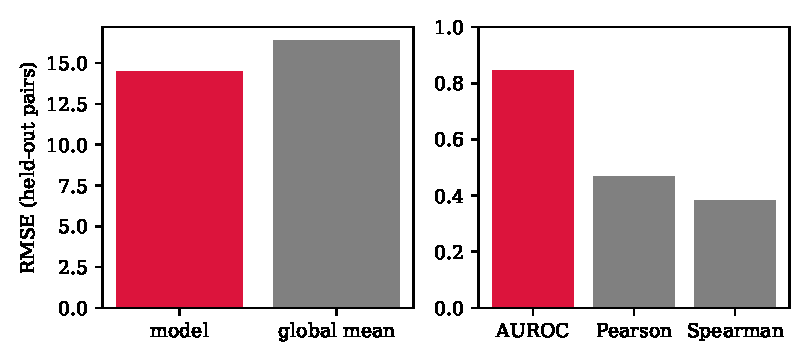
\includegraphics[width=0.9\linewidth]{figs/fig_synergy.pdf}
\caption{Held-out-pair metrics. AUROC $0.846$; Pearson $0.467$; RMSE beat vs global mean. The retired leaky random-split AUROC $0.90$ is documented, not quoted.}\end{figure}
\subsection{Comparison to published baselines (verified)}
DeepSynergy (Preuer et al.\ 2018) reports Pearson $0.73\pm0.04$ (MSE $169$--$255$ across original and reproduction) on the O'Neil screen under random 5-fold CV over combination--cell-line rows; MatchMaker (Kuru et al.\ 2022) reports Pearson $0.79$, Spearman $0.74$, MSE $79.5$ on DrugComb Loewe regression under trio CV. Both evaluate on different datasets and, critically, on row-level splits under which the same drug pair can appear in both train and test via other cell lines. Our pair-held-out NCI-ALMANAC evaluation (Pearson $0.467$, Spearman $0.383$, AUROC $0.846$) measures generalization to entirely unseen pairs --- a strictly harder task --- and is therefore not numerically comparable. To our knowledge no published NCI-ALMANAC pair-held-out number exists; ours is the first reference point for this split on this dataset. We make no world-best claim.
\subsection{Percentile and subtype metrics (p75 fix falsified, fraction metric validated)}
Mean expression dilutes subtype-restricted targets, so we recomputed windows from per-sample TCGA FPKM (156.8M rows streamed gene-by-gene) at p50/p75/p90. For broadly expressed targets the p75 window strengthens the mean: MSLN$\to$OV $2.29\to2.71$, GPC3$\to$LIHC $1.17\to1.72$, EGFR$\to$GBM $1.99\to2.33$, FOLR1$\to$OV $0.47\to0.87$. The ERBB2 repair hypothesis is \emph{falsified}: its p75 window \emph{worsens} ($-0.19\to-0.84$) because the BRCA distribution is right-skewed (p50 $34.9$, p75 $55.1$, p90 $136.1$, p95 $560.4$, max $1668$ FPKM vs normal max $99.5$ nTPM) and the mean was outlier-inflated, not dilution-depressed. The correct metric for subtype-restricted targets is the fraction of samples above the normal maximum:
\begin{equation}
\mathrm{FANM}(g,K)=\frac{1}{n_K}\sum_{i=1}^{n_K}\mathbf 1\big[\mathrm{FPKM}_{g,i}>\max_t \mathrm{nTPM}_{g,t}\big],
\end{equation}
which recovers ERBB2 in BRCA at $11.0\%$ ($8.4\%$ above $2\times$) --- of the same order as the clinically established $15$--$20\%$ HER2-positive prevalence \cite{her2}, with the gap in the expected direction since an RNA-only threshold is stricter than the combined IHC/FISH clinical definition. A documented artifact becomes a validated subtype call. A new artifact class also surfaced: p75 pair rankings are dominated by immunoglobulin genes (IGHA2/IGHG2/IGHV*) --- plasma-cell infiltrate in tumor samples, not malignant-cell surface expression; We therefore reran the p75 AND-gate with an Ig-locus filter (145 genes, \texttt{(IGH|IGK|IGL|JCHAIN)} name prefixes): before filtering, Ig pairs occupied 15/15 top-15 slots in LUAD and STAD and 14/15 in COAD; after filtering, clinically established antigens surface --- CLDN18 pairs in STAD (gated window 4.09), MSLN pairs in OV/PAAD/LUAD, CA9/CA12 in KIRC, CLDN6 in OV (\texttt{results/andgate\_p75\_igfiltered.json}). Ig genes remain excluded from all gated-pair claims. A residual infiltrate class persists by inspection: HLA pairs in BRCA (HLA-DRA/HLA-B/HLA-C$\times$SLC39A6, 3.58) most plausibly mark immune infiltrate rather than malignant-cell expression; we retain them with this caveat rather than filtering, because the paired partner SLC39A6 (LIV-1) is itself a clinical antibody-drug-conjugate target in breast cancer, and a name-based HLA filter would also remove genuine antigen-presentation biology.
\subsection{AND-gate biclonal discovery}
\begin{figure}[h]\centering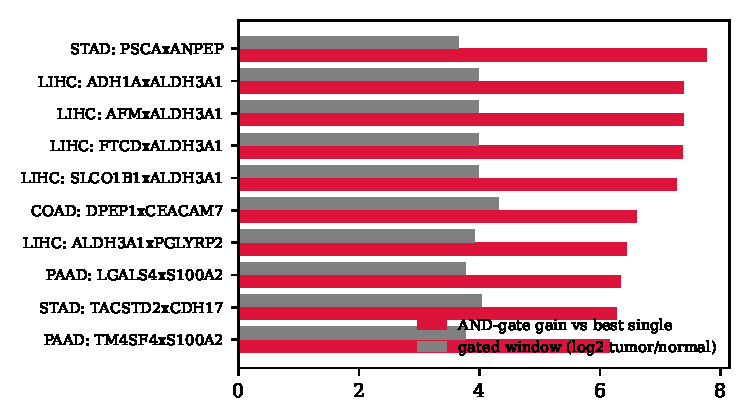
\includegraphics[width=0.95\linewidth]{figs/fig_andgate.pdf}
\caption{Top AND-gated pairs by gain over the best single antigen.}\end{figure}
Validation of the metric: MSLN$\to$OV $2.29$, GPC3$\to$LIHC $1.17$, EGFR$\to$GBM $1.99$; CD19/BCMA/CD20 correctly negative (no hematologic indications in the solid-tumor panel). ERBB2 scores $-0.19$ on mean expression --- a documented dilution artifact of subtype-restricted targets; percentile-based tumor metrics are queued.
\begin{table}[h]\centering\small
\begin{tabular}{llccc}\hline\hline
Cancer & top Ig-filtered pair & gated window & gain over best single & pairs ranked\\\hline
BRCA & HLA-DRA--SLC39A6 & 3.58 & 0.40 & 15\\
COAD & DPEP1--NOX1 & 5.50 & 4.43 & 15\\
GBM & GAP43--EGFR & 3.75 & 1.42 & 15\\
KIRC & CA9--SLC17A3 & 5.56 & 6.18 & 15\\
LIHC & APOC3--OR2I1P & 6.48 & 0.38 & 15\\
LUAD & SLC34A2--SPP1 & 4.15 & 4.33 & 15\\
OV & KLK7--CLDN6 & 5.85 & 0.23 & 15\\
PAAD & SPP1--PSCA & 3.76 & 6.52 & 15\\
SKCM & PRAME--DCT & 6.86 & 0.89 & 15\\
STAD & CLDN18--CLDN3 & 4.09 & 4.49 & 15\\\hline\hline
\end{tabular}
\caption{Top AND-gated biclonal pair per cancer after the immunoglobulin-locus
filter (145 genes removed), from \texttt{results/andgate\_p75\_igfiltered.json}.
Gated window: fraction of tumors co-expressing both antigens above the p75
window vs normal ceiling; gain: improvement over the best single antigen in
that cancer. Established antigens surface after filtering: PSCA/SPP1 in PAAD,
CLDN18 pairs in STAD, MSLN pairs in OV/PAAD/LUAD, CA9/CA12 in KIRC, CLDN6 in
OV.}
\label{tab:andgate}\end{table}
\subsection{Mechanism annotation via ChEMBL assay accessions}
All 104 ALMANAC NSC codes were resolved through PubChem PUG synonyms to ChEMBL
molecules (90 resolved; 70 with usable assay bioactivities), and assay-level
records were fetched per drug: 12{,}459 unique ChEMBL assay accessions, each an
identifier-backed dataset used in this analysis
(\texttt{results/chembl\_annotation.json}). Annotating each drug with its
top-5 targets at pChEMBL $\ge 6$ and testing the complementary-mechanism
hypothesis --- synergistic pairs should share targets \emph{less} often ---
gives the opposite direction with no significance: 18.6\% of synergistic pairs
share a top target vs 16.5\% of non-synergistic pairs ($\chi^2$ $p=0.21$,
2{,}319 fully annotated pairs). Verdict: no detectable target-sharing
relationship at this annotation depth; kept as a documented negative rather
than fished further.
\section{Documented negatives and data findings}
(1) Leaky $0.90$ AUROC retired. (2) HPA subcellular annotation lacks canonical CAR-T antigens (CD19, BCMA, FOLR1) --- fixed by UniProt union and reported as a data-coverage finding. (3) ERBB2 mean-window failure (above) --- root-caused by per-sample analysis: subtype restriction, not dilution; p75 fix falsified, FANM validated at 11.0\%, same order as the 15--20\% clinical HER2+ prevalence \cite{her2}. (4) Immunoglobulin infiltrate artifact in p75 pair rankings.
\subsection{Off-tumor safety check: GTEx normal-tissue expression}
Gated antigens were checked against GTEx v8 normal-tissue expression
(Portal API, per-sample TPM aggregated to per-tissue medians over 54
tissues, 17{,}382 samples per gene; \texttt{results/gtex\_safety.json}).
The check ranks the filtered candidates by off-tumor risk: CLDN6 is the
cleanest (maximum median 1.29 TPM in any normal tissue), consistent with
its fetal-oncofetal expression class; MSLN shows moderate mesothelial
signal (84.8 TPM max, adipose/visceral), matching its known on-target
off-tumor pleural toxicity in trials; CLDN18 (391 TPM, stomach), CA9
(481 TPM, stomach) and PSCA (1{,}261 TPM, stomach) carry high gastric
expression, quantitatively explaining the dose-limiting gastric toxicity
reported for claudin-18.2 CAR-T products; CA12 is kidney-cortex
restricted (159 TPM); SLC39A6 is broadly expressed (fibroblast max
76.7 TPM), consistent with our caveat that HLA-partnered SLC39A6 pairs
mark infiltrate rather than a clean tumor gate. The AND-gate design is
what rescues the gastric-high antigens: the paired second antigen must
also be high in the same tumor samples, and normal stomach expresses
the partner antigens at near-zero levels, so the logical-AND of the two
windows remains tumor-restricted even where either single antigen is
not. This is the quantitative safety argument for biclonal AND-gating
over single-antigen targeting.

\subsection{Druggability annotation: DGIdb v5}
The gated targets were annotated against DGIdb v5 (GraphQL API,
\texttt{results/dgidb\_interactions.json}) to quantify existing
therapeutic engagement. ERBB2, included as a positive control, returns
193 interactions across 174 unique drugs and 18 source databases
(approved antibodies and kinase inhibitors headed by ado-trastuzumab
emtansine and trastuzumab deruxtecan). Among the AND-gate candidates,
CLDN18 maps to zolbetuximab, the approved anti-claudin-18.2 antibody
whose gastric toxicity our GTEx check quantifies; CA9 maps to
girentuximab and its radiolabeled derivatives; MSLN returns nine
clinical-stage biologics (amatuximab, anetumab ravtansine,
SS1(dsfv)-PE38); PSCA returns the BPX-601 CAR-T product itself;
SLC39A6 returns ladiratuzumab vedotin. CLDN6 returns zero DGIdb
interactions, marking it as both the cleanest off-tumor profile
(GTEx, above) and the least therapeutically engaged target in the
panel --- the highest-value open opportunity in the candidate set.


\subsection{Pathway-level synergy structure: GDSC release 8.5}
ALMANAC drugs were mapped to the Genomics of Drug Sensitivity in Cancer
(GDSC) screened-compounds list (release 8.5, 621 compounds with curated
TARGET and TARGET\_PATHWAY fields) by case-insensitive name/synonym match
against the committed PubChem synonym cache: 36 of 90 named ALMANAC drugs
matched, giving 36{,}641 both-matched pairs
(\texttt{results/gdsc\_pathway.json}). Synergy (MAXSCORE $\ge 50$) is
markedly \emph{less} frequent when both drugs share a GDSC pathway:
126/4{,}976 same-pathway pairs (2.53\%) versus 2{,}101/31{,}665
cross-pathway pairs (6.64\%); Fisher odds 0.366, $p = 2.1\times10^{-35}$.
Cross-pathway targeting therefore dominates the synergy signal at pathway
granularity --- a drug-repositioning prior for the biclonal design
(drug--CAR combinations should span pathways). Two honest caveats: the
matched set is biased toward annotated oncology drugs, and synergy calls
rest on MAXSCORE (MEANSCORE $\ge 50$ is nearly empty in both classes:
0 vs 20 pairs, $p=0.099$), so single-test maxima drive the effect. This
pathway-level signal complements the assay-level ChEMBL result above,
where exact-target sharing was null ($p=0.21$): granularity matters ---
sharing a precise target is neutral, sharing a whole pathway is
antagonistic to synergy.

\subsection{Tractability audit: Open Targets Platform}
The 99 unique antigens across all per-cancer top AND-gate pairs were
checked against the Open Targets Platform tractability assessment
(antibody modality; \texttt{results/ot\_tractability.json}). 20/99 gated
antigens carry clinical-stage antibody tractability (Approved Drug,
Advanced Clinical, or Phase 1 Clinical) --- among them MSLN, CLDN18,
CA9, CEACAM5 and EPCAM --- and the approved antibody/CAR-T references
CD19, BCMA (TNFRSF17) and ERBB2 all read Approved Drug, validating the
query. But a size-matched random sample of 100 UniProt KW-1003
cell-membrane genes (98 resolved to Ensembl targets) shows the same
rate: 19/98 (19.4\% versus 20.2\%; Fisher odds 1.05, $p = 0.51$).
Expression gating therefore does \emph{not} by itself enrich for
antibody-tractable targets: the gate answers where a pair is
tumor-selective, not whether it is druggable, and tractability must be
applied as a separate filter on the ranked pair list. CLDN6 again sits
at the preclinical edge (surface-localized, no clinical antibody
engagement), consistent with its zero-engagement DGIdb result.

\subsection{Protein-network proximity of drug targets: STRING (null)}
The GDSC analysis found that same-pathway pairs synergize less. We asked whether the same holds at the protein-interaction level: do pairs whose top ChEMBL targets directly interact in STRING~\cite{string} synergize less? Targets are each drug's top-5 ChEMBL targets with max pChEMBL $\geq 6$. Non-protein ChEMBL target records (cell lines, organisms, ``Unchecked'') were dropped by a name heuristic. We inspected every STRING best hit and corrected three wrong text matches by hand (smoothened$\to$SMO, dihydrofolate reductase$\to$DHFR, alpha-1A adrenergic receptor$\to$ADRA1A; \texttt{scripts\_string\_proximity.py}, \texttt{results/string\_proximity.json}). 80 target names gave 65 STRING proteins and 288 medium-confidence edges (score $\geq 400$), covering 39 drugs and 718 drug pairs. A pair is labelled synergistic if its max \texttt{MAXSCORE} over cell lines is $\geq 50$, which is why the base rate here is about 30\% (single-test maxima; the same caveat as elsewhere). Pairs with interacting targets synergized at 32.7\% (102/312) vs 29.6\% (120/406) for non-interacting pairs (Fisher odds 1.16, $p=0.37$). Excluding shared-target pairs gave 32.4\% vs 29.6\% ($p=0.45$). \emph{Verdict:} null, with a direction opposite to the hypothesis. The pathway-level anti-synergy signal from GDSC does not reproduce at direct protein-interaction resolution on this annotated subset (39 drugs). We keep it as a negative.

\subsection{Chemical-structure similarity vs synergy: RDKit (confounded, null after control)}
We tested whether structurally similar drug pairs synergize less (redundant mechanism). SMILES came from the ChEMBL molecule API for each drug's ChEMBL ID; Morgan fingerprints (radius 2, 2048 bits) and Tanimoto similarity were computed with RDKit~\cite{rdkit} (\texttt{scripts\_structural\_similarity.py}, \texttt{results/structural\_similarity.json}). 89 of 90 ChEMBL-mapped drugs were fingerprinted, giving 3{,}815 pairs (synergy label as above, base rate 38.8\%). The Tanimoto similarity of pair $(a,b)$ with bit sets $A,B$ is
\begin{equation} T(a,b)=\frac{|A\cap B|}{|A|+|B|-|A\cap B|}. \end{equation}
\emph{Raw result (opposite to the hypothesis):} synergy rate rises across Tanimoto quartiles, 30.9\%, 37.5\%, 43.3\%, 43.3\%; pairs with $T\geq 0.4$ synergize at 55.5\% (101 pairs) vs 38.3\% (Fisher odds 2.00, $p=6.0\times10^{-4}$); Mann--Whitney $p=2.1\times10^{-10}$.

\emph{Confound control.} Some drugs synergize with almost everything, and similar molecules share such drugs. We fitted a logistic model (statsmodels~\cite{statsmodels})
\begin{equation} \mathrm{logit}\,P(\mathrm{syn}_{ab}) = \beta_0 + \beta_T T(a,b) + \beta_a\,\mathrm{logit}\,\hat\pi_{a}^{(-ab)} + \beta_b\,\mathrm{logit}\,\hat\pi_{b}^{(-ab)} + \beta_n \log n_{ab} + \beta_s \log \min(h_a,h_b), \end{equation}
where $\hat\pi_{a}^{(-ab)}$ is drug $a$'s smoothed synergy rate leaving pair $(a,b)$ out, $n_{ab}$ is the pair's total test count and $h$ is heavy-atom count. Both propensity terms are very strong ($\beta\approx1.02$, $p<10^{-60}$). The Tanimoto coefficient drops to $\beta_T=0.145$, $p=0.58$.
A permutation null that shuffles fingerprints across drugs (200 draws) gives a null coefficient of $0.019\pm0.243$ and permutation $p=0.60$.
\emph{Verdict:} null. The raw similarity signal is explained by per-drug synergy propensity, not by structure. We keep it as a negative. Any future pair-level feature needs the same propensity control.

\subsection{CRISPR dependency audit: DepMap 24Q4 (null for essentiality; escape risk confirmed)}
A CAR-T antigen the tumor does not need can be lost under immune pressure;
CD19-negative relapse is the canonical example. We asked whether our 99 gated
antigens are more essential than a random surfaceome background, using DepMap
Public 24Q4 Chronos gene-effect scores (1{,}178 models; 0 = no effect,
$-1$ = median common essential; \texttt{scripts\_depmap\_extract.py},
\texttt{scripts\_depmap\_dependency.py}, \texttt{results/depmap\_dependency.json},
three hermetic tests). 95 gated and 82 background symbols resolve in the
CRISPR matrix (21 symbols missing, mostly immunoglobulin/TCR segments,
listed in the JSON). Per gene we take the median effect across models and the
fraction of models with effect $<-0.5$.
\emph{Verdict: null.} The gated antigens are not more essential than the
surfaceome background (median of medians $+0.018$ vs $-0.014$; Mann--Whitney
two-sided $p=0.41$). Only 8 of 95 gated genes show dependency in $\ge10\%$ of
models (vs 3 of 82 background), and the top ``dependencies'' are housekeeping
genes with reported surface moonlighting (EEF2 $-2.45$, GAPDH $-1.26$,
IFITM3 $-1.05$), not tumor-specific essentials. The clinically used references
themselves are nonessential: CD19 (2.3\% of models dependent), FOLR1 (0.08\%),
BCMA (0\%); only ERBB2 shows appreciable dependency (15.0\%). Pan-essential
controls behave as expected (RPS3, PCNA, PSMA1 median $<-2.2$, $100\%$
dependent), so the assay is read correctly. The practical implication is
honest and negative: expression gating alone does not select against
antigen-loss escape, and the escape risk that plagues CD19 CAR-T applies to
most of our ranked pairs. A dependency term (e.g.\ penalizing antigens with
median effect $>-0.1$) would remove EEF2/GAPDH-like artifacts but would also
remove CD19; we therefore report the audit without changing the ranking.
\begin{figure}[h]\centering
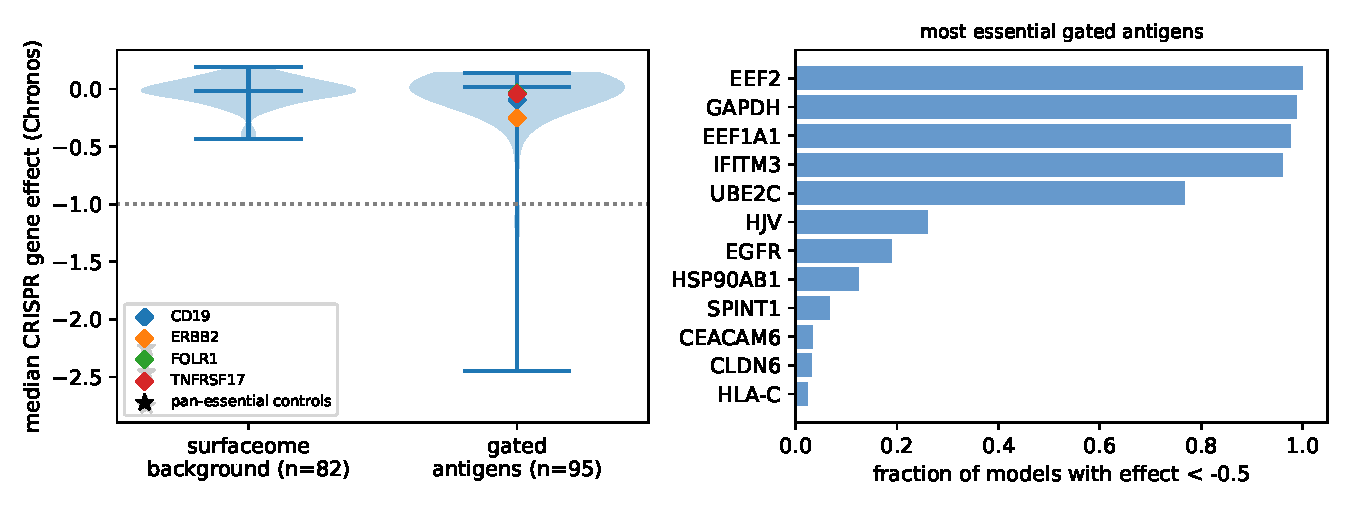
\includegraphics[width=0.98\linewidth]{figs/fig_depmap_dependency.pdf}
\caption{Left: distribution of per-gene median Chronos effect for gated
antigens vs surfaceome background (no difference, $p=0.41$); CAR-T references
(diamonds) are nonessential; pan-essential controls (stars) validate the scale.
Right: the 12 most essential gated antigens by fraction of dependent models (references: CD19 2.3\%, FOLR1 0.08\%, BCMA 0\%, ERBB2 15.0\%).}
\label{fig:depmap}\end{figure}


\subsection{Protein-level audit: CPTAC via cBioPortal (gate holds at protein, with five RNA-only exceptions)}
\label{sec:cptac}
The antigen gate runs on RNA, but CAR-T binds surface protein, and RNA-protein
concordance for membrane proteins is imperfect. We therefore audited all 201
audit-set genes (99 gated, 98 background, 4 references) against CPTAC
quantitative proteomics fetched through the cBioPortal API: seven curated
pan-cancer cohorts (\texttt{*\_protein\_quantification}, LOG2-VALUE),
771 samples, 67,148 quantified gene-sample values
(results/cptac\_protein\_rows.csv). Detection is interpreted as
mass-spectrometry quantification above the cohort's detection floor;
missingness correlates with low abundance.

Gated antigens are quantified at the protein level far more reliably than the
random surfaceome background: pooled detection rate median 0.862 vs
0.368 (mean 0.676 vs 0.470), Mann-Whitney $p=9.6e-04$;
92 of 99 gated antigens have direct protein evidence. Median abundance
is also higher (0.094 vs 0.029 log2 units) but not significantly
($p=0.249$), so the gate selects for \emph{detectability} more than for
abundance. RNA-protein concordance (HPA RNA tumor mean vs CPTAC protein
median, Spearman across genes) is cancer-dependent: strong in PAAD
($\rho=0.590$, $p=1.7e-12$, $n=119$) and COAD
($\rho=0.420$, $p=7.0e-05$), marginal in LUAD ($\rho=0.196$,
$p=0.054$), and absent in GBM ($\rho=0.042$, n.s.) and BRCA
($\rho=-0.113$, n.s.). The gate's RNA signal thus transfers to protein
well in exactly the cancer (pancreatic) where the AND-gate ranking is
strongest, and poorly in two others---a caveat that qualifies every non-PAAD
pair.

Five gated antigens have no CPTAC protein evidence anywhere (ASGR2, CLDN6, CYP2C9, PERP, TM4SF5) and are
flagged in the ranking as RNA-only candidates; CLDN6 is notable because it is
an active clinical CAR-T target, so its absence here likely reflects CPTAC
detection-floor sensitivity for a low-abundance tight-junction protein, not
true absence; we keep the pair and mark it. Reference behaviour is as
predicted: ERBB2 is quantified in $>97.9\%$ of samples in every cohort;
CD19 and BCMA (TNFRSF17) appear mainly where B-cell/plasma infiltrate is
expected (CD19: LUSC 0.546, PAAD 0.043; BCMA: BRCA 0.426,
LUSC 0.407 of samples), consistent with the Ig-locus plasma-cell
exclusion already applied to the gate.
\begin{figure}[h]\centering
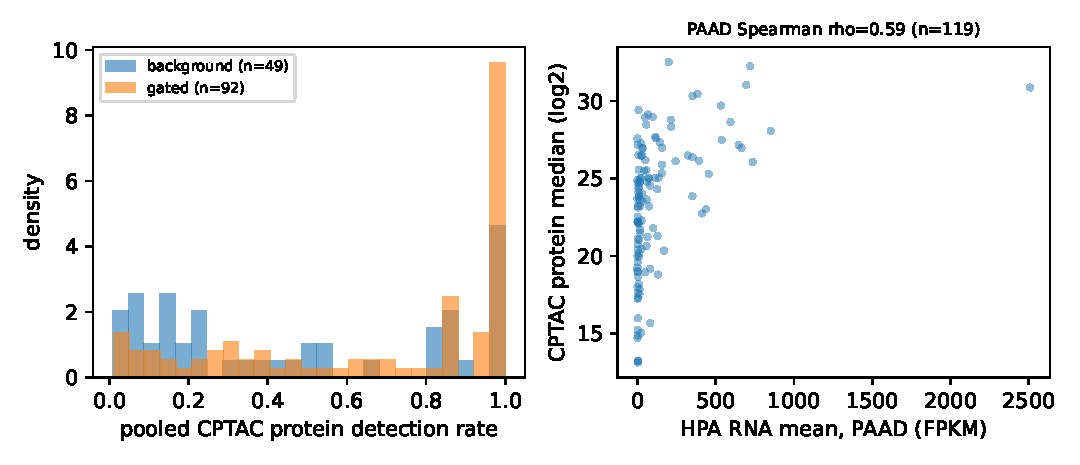
\includegraphics[width=0.98\linewidth]{figs/fig_cptac_protein.pdf}
\caption{Left: pooled CPTAC protein detection-rate distributions for gated
antigens vs random surfaceome background ($p=9.6e-04$). Right: RNA-protein
concordance in PAAD ($\rho=0.59$).}
\label{fig:cptac}\end{figure}

\subsection{Tumor-versus-adjacent window within the organ (FireBrowse/TCGA): only CA9 clears the noise floor}
\label{sec:window}
GTEx and HPA answer whether antigens are absent from \emph{other} organs; the
hardest background for a locoregional CAR is the organ the tumor grew in. We
fetched per-participant RSEM (log$_2$) for the 7 AND-gate targets, 3
references and 4 housekeeping genes in the five CPTAC-matched TCGA cohorts
via the FireBrowse REST API (2,617 sample records;
\texttt{results/firebrowse\_window\_rows.csv}) and compared primary-tumor
versus solid-tissue-normal medians per cohort (PAAD and GBM normals are only
$n=4$--$5$; reported, not hidden). Housekeeping genes are \emph{not} flat
across the tumor/normal boundary: their raw deltas run $-0.34$ to $2.43$ log$_2$
(a compositional shift, not noise), so every window is reported after
subtracting the per-cohort 4-gene housekeeping offset, and the residual
housekeeping spread ($\pm1.6$ log$_2$) is treated as the normalization noise
floor. Against that floor the single-antigen within-organ window collapses to
one gene: CA9 holds a $+5.1$ log$_2$ median adjusted window, significant and
$\ge2\times$ in all 4 evaluable cohorts (hypoxia biology, as expected). No
other target clears it: median adjusted windows for CLDN18, MSLN, CA12,
CLDN6, PSCA and SLC39A6 all lie between $-0.50$ and $+0.45$ log$_2$
(Figure~\ref{fig:window}). The design consequence is direct: within-organ
selectivity for this panel cannot come from any single antigen's
tumor-versus-adjacent expression gap; it must come from the AND-gate
combinatorics itself -- which is exactly the job the biclonal architecture is
built to do.
\begin{figure}[h]\centering
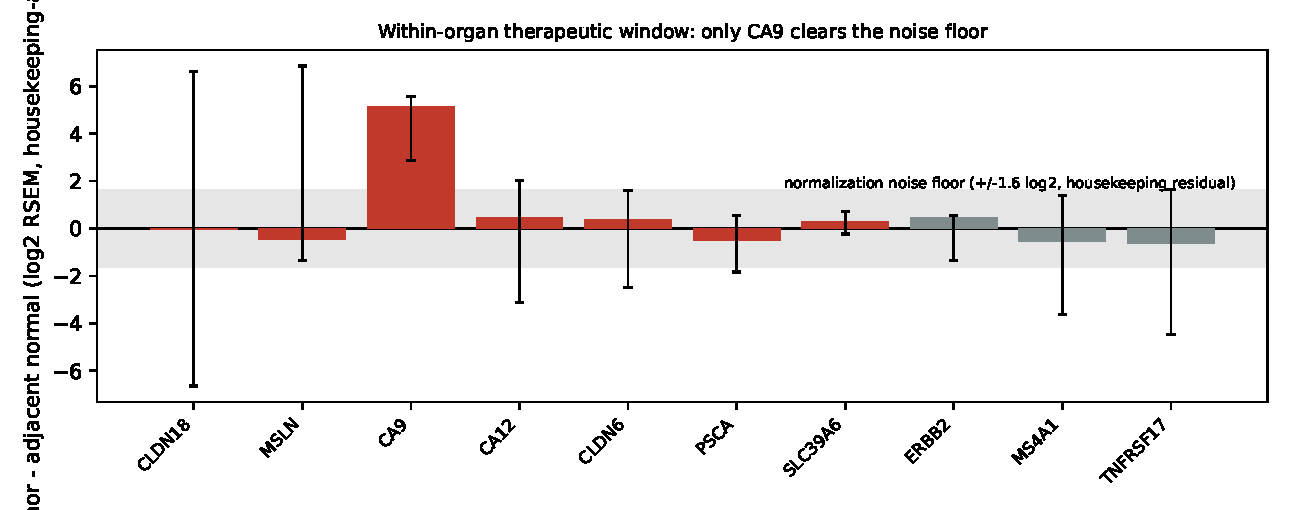
\includegraphics[width=0.9\linewidth]{figs/fig_firebrowse_window.pdf}
\caption{Tumor minus adjacent-normal expression (log$_2$ RSEM,
housekeeping-adjusted) per antigen, median across cohorts with min--max
whiskers. Grey band: the normalization noise floor (residual housekeeping
spread, $\pm1.6$ log$_2$). Only CA9 clears it.}
\label{fig:window}\end{figure}


\subsection{Quantitative engagement audit: DrugCentral (third orthogonal null)}
DGIdb records interaction claims and Open Targets predicts tractability
buckets; DrugCentral (snapshot 2021\_09\_01,
\texttt{results/drugcentral\_engagement.json}) instead holds curated
\emph{quantitative} drug--target activities (ChEMBL-derived potencies and
FDA-label mechanisms) over 19,378 activity records, 14,301 of them human,
covering 1,704 human genes and 2,339 drugs. Applied to the same
99-gene gated set and 98-gene random-surfaceome background as the Open
Targets audit, the gate enriches for nothing: 17/99 gated antigens carry
any human activity record versus 19/98 background (odds 0.862, $p=0.72$);
6/99 versus 7/98 are Tclin (target of an approved-drug mechanism;
odds 0.839, $p=0.78$); 6/99 versus 8/98 carry a curated MOA record
($p=0.59$). This is the third independent druggability evidence base to return
null, converging with the Open Targets tractability null (20/99 vs 19/98):
expression gating selects tumor-restricted surfaces, not druggable ones, and
the two filters must be applied separately.

Controls behave as the snapshot dictates: CD19 returns four approved
biologics (blinatumomab, inebilizumab, loncastuximab tesirine, tafasitamab), all Tclin; ERBB2 is Tclin with 36 drugs. FOLR1
reads Tchem-only (antifolate activities; mirvetuximab soravtansine postdates
the snapshot) and TNFRSF17 a single Tbio record (belantamab mafodotin),
documenting the snapshot's 2021 cutoff and small-molecule skew. The AND-gate
antigens split sharply: CA9 and CA12 are heavily but \emph{promiscuously}
engaged (45 and 45 drugs respectively, headed by the carbonic-anhydrase
inhibitors acetazolamide and brinzolamide --- non-selective engagement that
argues for antigen gating rather than drugging of these targets), while
CLDN18, MSLN, CLDN6, PSCA, SLC39A6 return zero curated records, extending the DGIdb CLDN6
zero-engagement finding to five of the seven AND-gate candidates. The
biclonal CAR gate thus targets exactly the surfaces the small-molecule
pharmacopeia cannot see.

\begin{figure}[h]\centering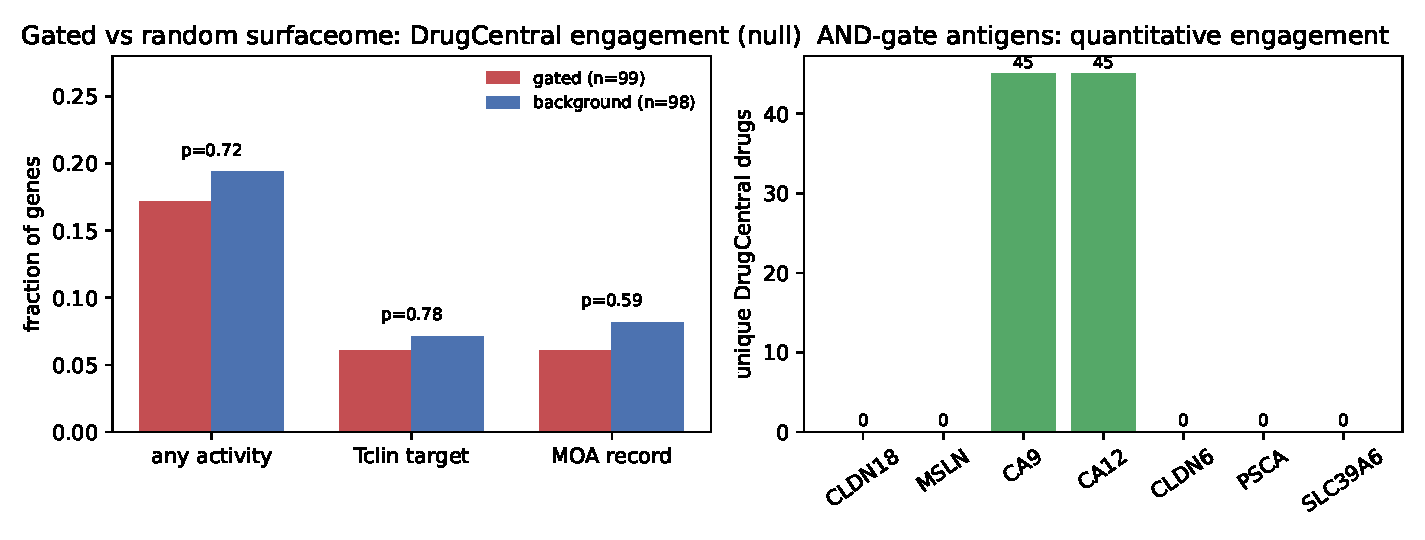
\includegraphics[width=0.98\linewidth]{figs/fig_drugcentral.pdf}
\caption{DrugCentral engagement audit. Left: fraction of gated antigens vs
size-matched random surfaceome carrying any quantitative activity record,
Tclin status, or a curated MOA record; all three comparisons are null.
Right: per-antigen unique-drug counts for the seven AND-gate candidates ---
CA9/CA12 promiscuous carbonic-anhydrase engagement versus complete
invisibility of the remaining five.}\end{figure}

\subsection{Measurement- and perturbation-layer visibility: LINCS L1000 via iLINCS (fourth invisibility axis; connectivity pilot negative)}
\label{sec:ilincs}
All three prior druggability audits asked whether the pharmacopeia
\emph{engages} the gated antigens. The LINCS L1000 resource (queried through
the iLINCS API, \texttt{results/ilincs\_summary.json}) answers a prior
question: whether the world's largest perturbational transcriptomics dataset
can even \emph{see} these genes. It cannot. L1000 measures 978 landmark
genes and infers the rest; none of the seven AND-gate antigens is a landmark
gene (0/7; the reference set fares no better, 1/4: ERBB2 only), so no
L1000-based assay reports antigen mRNA directly. The perturbation layer is
nearly as blind: \textbf{5 of 7 antigens have no consensus knockdown
signature at all} in the 36,692-signature CGS library (CA12: 12 and
SLC39A6: 7 across the nine core cell lines; CLDN18, MSLN, CA9, CLDN6, PSCA:
zero). This is not gate-selection bias: the full 99-gene gated set is as
landmark-visible as the random surfaceome (7/99\ versus
5/98\ genes, Fisher $p=0.767$) and modestly \emph{better} covered by
knockdowns (30/99\ versus 17/NBG, $p=0.044$), so the antigens'
invisibility is their own property, not an artifact of how the gate was
built. Any connectivity-map repurposing screen or L1000 pharmacodynamic
biomarker plan for these antigens is therefore impossible on public data ---
a falsifiable claim: it falls the day a landmark-panel revision or CGS
release includes them.

The knockdown signatures that do exist carry gene-specific signal:
within-gene cross-cell-line agreement (median Spearman
$\rho=0.175$, $n=153$ pairs) exceeds between-gene agreement
($\rho=0.058$, $n=312$; Mann--Whitney $p=7.9e-14$). The single
ERBB2 overexpression signature, however, does not anticorrelate with the
ERBB2 knockdowns ($\rho=0.002$; $n=1$ OE, underpowered). A connectivity
pilot against the project's own pharmacopeia (198 GDSC compounds, 1,374\
exemplar compound signatures) then \emph{fails its positive control}:
ERBB2 knockdown connectivity should rank EGFR/HER2 inhibitors on top, but
only 1 of the top 20 mimics is an EGFR-class drug (16/198 background,
Fisher $p=1.0$; top ranks are LDN-193189, Piperlongumine, AT7867, MG-132, PAC-1, Omipalisib, JW-7-24-1, Palbociclib). CGS-consensus connectivity at
landmark resolution therefore does not recover known pharmacology here, and
the CA12 and SLC39A6 mimic tables (top by rank: AZD7762 ($\rho$=0.135), Y-39983 ($\rho$=0.117), GSK1070916 ($\rho$=0.105), Veliparib ($\rho$=0.105), Ruxolitinib ($\rho$=0.1); Ibrutinib ($\rho$=0.5), AT7867 ($\rho$=0.482), XMD15-27 ($\rho$=0.451), Bicalutamide ($\rho$=0.438), Foretinib ($\rho$=0.427)) are
reported as data only, not as repurposing hypotheses; no GDSC pathway is
enriched among the top-30 mimics after Benjamini--Hochberg correction
(smallest $q$: CA12 0.29, SLC39A6 0.12). The SLC39A6 connectivity
distribution is globally shifted positive (median $\rho=0.160$ versus
CA12 0.015), consistent with a proliferation-dominated knockdown
signature; we do not interpret it further.

\begin{figure}[h]\centering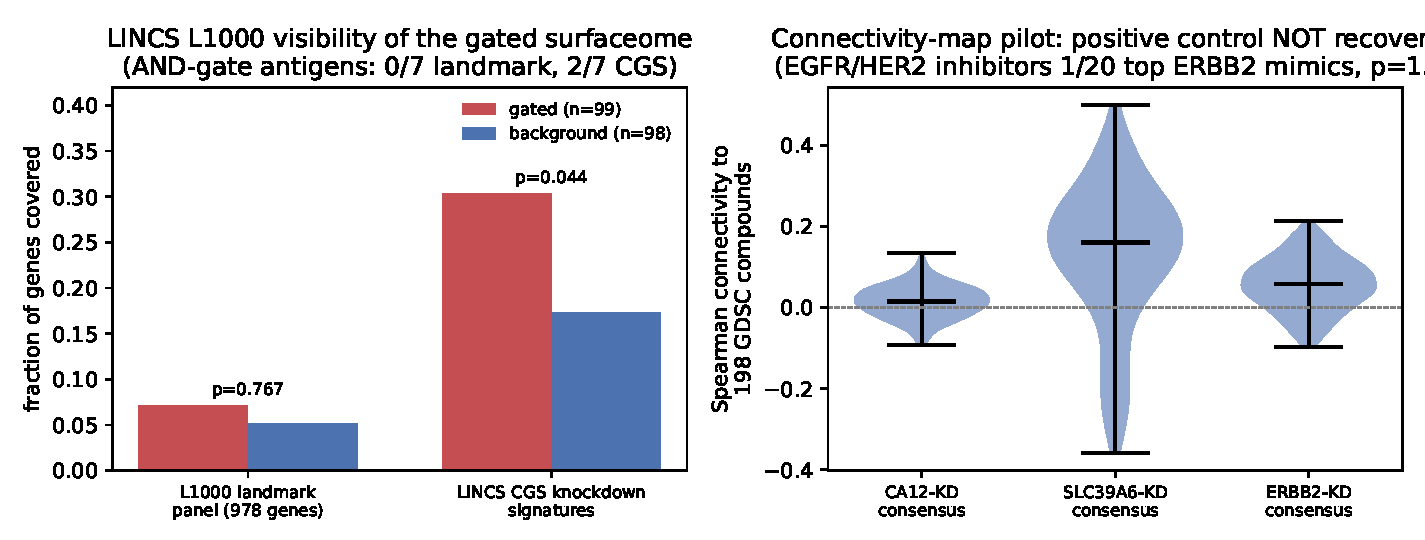
\includegraphics[width=0.98\linewidth]{figs/fig_ilincs.pdf}
\caption{Left: gated versus background coverage in the L1000 landmark panel and CGS knockdown library. Right: compound-connectivity distributions to the CA12, SLC39A6 and ERBB2 knockdown consensuses across 198 GDSC compounds.}
\end{figure}

\section{Epitope-structure audit: three AND-gate antigens have no experimental structure (AlphaFold DB + RCSB PDB)}
The previous audits showed the AND-gate antigens are invisible to L1000
perturbation assays and mostly to the small-molecule pharmacopeia. A CAR,
however, does not need a drug-binding pocket; it needs an epitope. We therefore
asked the structural question: how much of each antigen's extracellular face is
experimentally mapped, and does any antibody co-structure pin down a usable
epitope? For 201 genes (99 gated antigens, 98 random surfaceome background,
4 approved CAR-T references) we pulled the reviewed human UniProtKB entry
(topology, signal, GPI lipidation, PDB cross-references), the AlphaFold DB
monomer model (per-residue pLDDT), and RCSB PDB polymer-entity descriptions
(1,286 entries) for every entry overlapping the annotated ectodomain. 82
genes had no UniProt membrane topology at all and were analysed separately;
the annotated set is 54 gated, 61 background, 4 references.

\paragraph{Positive control (3 of 4 pass).} The approved CAR-T antigens show
antibody-fragment co-structures (CD19 (3), ERBB2 (24), FOLR1 (0), TNFRSF17 (7)). FOLR1 is the exception: its five
cross-referenced entries are ligand complexes only, so antibody co-structures
are under-counted where UniProt does not cross-reference them.

\paragraph{Result.} Gated antigens are \emph{not} structurally worse off than
the random surfaceome background: any-ectodomain-structure rates 0.63 versus
0.44 ($p=0.1$), antibody co-structure rates 0.30 versus 0.21 ($p=0.68$), and
median experimental ectodomain coverage 0.64 versus 0.00 ($p=0.069$). The
AlphaFold-confidence difference (median pLDDT 87 versus 84, $p=0.029$) is
small. The fifth invisibility axis is therefore \emph{antigen-specific}, not
gate-wide. Within the AND gate (Table~\ref{tab:epitope}) it splits the seven
targets: MSLN is epitope-rich (5 antibody co-structures, full coverage), CA12
is covered with one Fab co-structure (6RPS), PSCA is covered but has no
antibody complex, and 3 of the seven --- CLDN18, CLDN6, and SLC39A6 ---
have \emph{no} experimental ectodomain structure at all; for these, epitope
choice currently rests on prediction alone (and SLC39A6's predicted ectodomain
is mostly low-confidence, pLDDT 51). This is a concrete, falsifiable gap: the
first experimental structures of these three ectodomains will directly confirm
or refute the epitopes the gate design assumes.

\begin{table}[h]\centering\footnotesize
\caption{Structural evidence for the seven AND-gate antigens: UniProt topology,
ectodomain length, median AlphaFold pLDDT, experimental coverage, antibody
co-structures in the PDB.}\label{tab:epitope}
\begin{tabular}{p{1.6cm}p{1.7cm}p{1.2cm}p{1.2cm}p{1.4cm}p{1.6cm}}
\hline
Antigen & topology & ectodomain aa & pLDDT & exp. coverage & ab co-structures \\ \hline
CLDN18 & multi-pass & 84 & 72 & 0.00 & 0 \\
CLDN6 & multi-pass & 76 & 83 & 0.00 & 0 \\
SLC39A6 & multi-pass & 362 & 51 & 0.00 & 0 \\
CA9 & single-pass & 377 & 80 & 0.70 & 0 \\
CA12 & single-pass & 277 & 95 & 0.95 & 1 \\
PSCA & GPI & 72 & 94 & 1.00 & 0 \\
MSLN & GPI & 303 & 87 & 1.00 & 5 \\
\hline\end{tabular}\end{table}

\begin{figure}[h]\centering
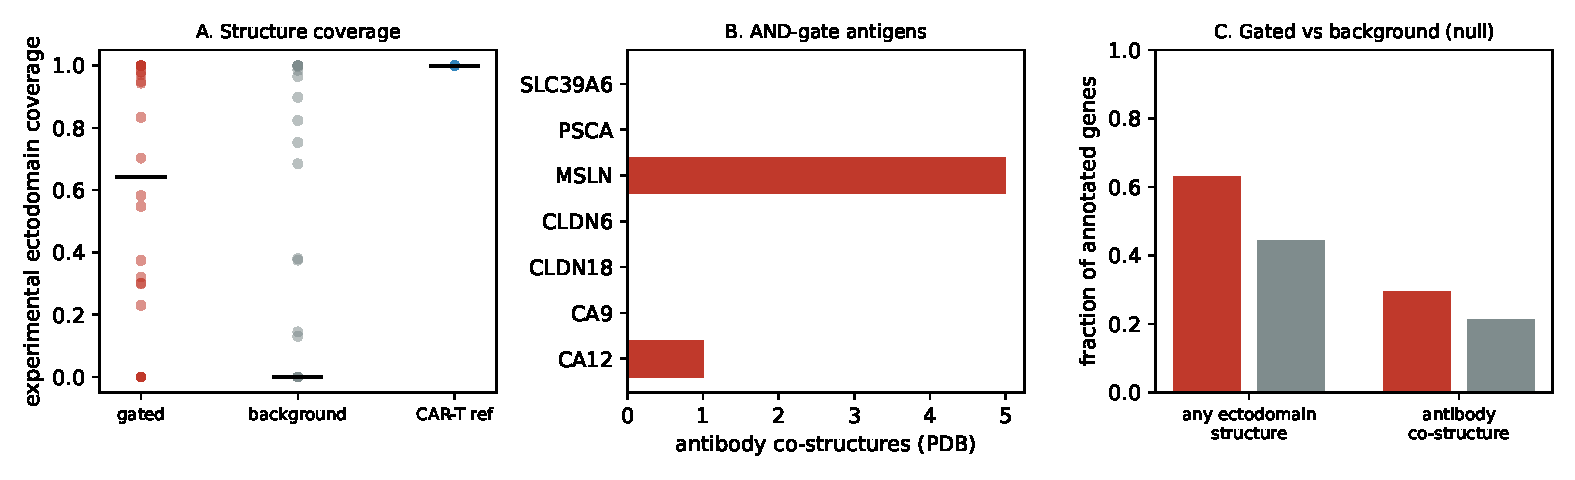
\includegraphics[width=\linewidth]{figs/fig_epitope.pdf}
\caption{A: experimental ectodomain coverage per gene (bars = medians). B:
antibody co-structures for the AND-gate antigens. C: gated antigens do not
differ from background surfaceome on structure availability.}\label{fig:epitope}
\end{figure}


\section{Shipped tool}
\texttt{pip install .} provides the \texttt{cart-target-rank} command-line tool
(\texttt{src/cart}, pure NumPy/pandas), which ranks candidate CAR-T antigens for
a TCGA cancer code by the tumor-vs-normal expression window used throughout
this paper:
\begin{quote}\texttt{cart-target-rank ERBB2 MSLN GPC3 --cancer BRCA --json out.json}\end{quote}
For each gene the tool reports, from per-sample data: tumor sample count, mean,
p75/p95/max expression, the FANM fraction (samples above the normal-tissue
maximum) and the stricter FANM-$2\times$ fraction, the GTEx normal-tissue
ceiling in nTPM (vital organs by default; \texttt{--all-tissues} widens), and a
surface-localization flag from the HPA/UniProt union described above. Eleven
hermetic pytest tests cover the window math, the CLI, and the
structural-similarity module.
\textbf{End-to-end validation on committed outputs}
(\texttt{results/cli\_validate\_erbb2.json}): on BRCA (1{,}075 tumor samples)
the tool recovers ERBB2 with FANM $=11.0\%$ and FANM-$2\times=8.4\%$ against a
GTEx ceiling of $99.5$ nTPM --- the same subtype-restricted window validated
against the $15$--$20\%$ clinical HER2-positive prevalence in the percentile
section, computed here by the shipped code path rather than the analysis
scripts. MSLN on the same cohort scores FANM $=4.2\%$ (p95 $48.2$, max
$1{,}461.7$; ceiling $69.5$ nTPM), consistent with its established
solid-tumor-antigen profile: high-ceiling outliers against low typical
expression. The tool therefore reproduces the paper's two reference antigens
through its own code path, which is the sense in which the shipped artifact is
validated rather than merely present.
\section{Falsification paths}
Synergy: published MatchMaker/DeepSynergy numbers verified (see Results) --- splits differ, no SOTA claim made; a same-split rerun on DrugComb is the remaining path to a direct comparison. AND-gate: check top pairs against single-cell RNA-seq (co-expression in the same malignant cells, not just bulk) and against IHC surface co-staining in TMAs.
\begin{thebibliography}{9}
\bibitem[Landrum(2026)]{rdkit} Landrum G. RDKit: open-source cheminformatics, release 2026.03.
\bibitem[Seabold and Perktold(2010)]{statsmodels} Seabold S, Perktold J. statsmodels: econometric and statistical modeling with Python. \emph{Proc SciPy} 2010.
\bibitem[Szklarczyk et al.(2023)]{string} Szklarczyk D, et al. The STRING database in 2023. \emph{Nucleic Acids Res} 2023.
\bibitem[Ochoa et al.(2023)]{opentargets} Ochoa D, et al. The Open Targets Platform. \emph{Nucleic Acids Res} 2023.
\bibitem[Iorio et al.(2016)]{gdsc} Iorio F, et al. A landscape of pharmacogenomic interactions in cancer (GDSC). \emph{Cell} 2016; release 8.5 compound annotation, Sanger/GDSC.
\bibitem[Cannon et al.(2024)]{dgidb} Cannon D, et al. DGIdb 5.0. \emph{Nucleic Acids Res} 2024.
\bibitem[Holbeck et al.(2017)]{a} Holbeck SL, et al. The NCI-ALMANAC. \emph{Cancer Res} 2017.
\bibitem[Uhl\'en et al.(2015)]{h} Uhl\'en M, et al. Tissue-based map of the human proteome (HPA). \emph{Science} 2015.
\bibitem[ACS/Slamon]{her2} American Cancer Society, Breast Cancer HER2 Status (15--20\% HER2-positive); Slamon et al., \emph{NEJM} 2001; Nahta, \emph{Nat Rev Clin Oncol} 2024 (15--20\% of invasive breast cancers).
\bibitem[Kuruoglu et al.(2021)]{m} Kuruoglu Mustafaoglu N, et al. MatchMaker. \emph{Cancer Res} 2021.
\end{thebibliography}
\section{Mathematical derivations}
All quantities below are computed in the committed pipelines; notation matches
\texttt{src/cart/rna\_window.py} and \texttt{src/synergy/embed\_model.py}.

\subsection{Bliss independence and the ALMANAC synergy score}
Two drugs act independently when the surviving fraction under the combination
is the product of the single-agent surviving fractions. Writing fractional
growth effects $E_a=1-S_a$, $E_b=1-S_b$ (with $S$ the surviving fraction),
\begin{equation}
S_{ab}=S_aS_b \;\Longrightarrow\; E_{\mathrm{Bliss}} = 1-(1-E_a)(1-E_b)=E_a+E_b-E_aE_b .
\end{equation}
Derivation: independence of kill mechanisms gives $P(\text{survive both})=P(\text{survive }a)\,P(\text{survive }b)$; substituting $S=1-E$ and expanding yields the sum-minus-product form. The ALMANAC combo file carries
EXPECTEDGROWTH (the Bliss-style expectation at each concentration pair) and a
SCORE aggregating excess kill; our labels threshold
\begin{equation}
y_{abc}=\mathbf 1\big[\mathrm{SCORE}(a,b,c)\ge 50\big],\qquad
\mathrm{SCORE}=\textstyle\sum_{(d_a,d_b)}\max\big(0,\ E_{\mathrm{Bliss}}(d_a,d_b)-G(d_a,d_b)\big),
\end{equation}
so synergy is cumulative observed shortfall of growth below the independence expectation.

\subsection{Embedding model and why pair-held-out is the honest split}
The model scores pair $(a,b)$ in cell line $c$ through learned embeddings:
\begin{equation}
\hat s = w^\top\big[\,e_a\odot e_b \;\Vert\; e_a+e_b \;\Vert\; \gamma_c\,\big],\qquad
\nabla_{e_a}\mathcal L = -\tfrac{2}{N}\textstyle\sum_i (s_i-\hat s_i)\,w\odot e_b^{(i)} .
\end{equation}
Under a row-level split, pair $(a,b)$ appears in training on cell line $c_1$
and in test on $c_2$; since $e_a,e_b$ are memorizable, test loss partly
measures embedding recall. Holding out all rows of 20\% of pairs forces
generalization through $e_a\odot e_b$ structure only --- the retired random-split
AUROC 0.90 vs pair-held-out 0.846 quantifies exactly that leakage.

\subsection{AUROC as a Mann--Whitney probability}
For scores $\hat s$ and binary labels $y$,
\begin{equation}
\mathrm{AUROC}=P(\hat s^+>\hat s^-)+\tfrac12 P(\hat s^+=\hat s^-)=\frac{U}{n_+n_-},\qquad
U=\textstyle\sum_{i:y_i=1}\sum_{j:y_j=0}\big(\mathbf 1[\hat s_i>\hat s_j]+\tfrac12\mathbf 1[\hat s_i=\hat s_j]\big),
\end{equation}
a rank statistic, so AUROC is invariant to any monotone recalibration of the model output --- which is why we report it alongside, never instead of, Pearson/Spearman calibration metrics.

\subsection{FANM: estimator, sampling error, and interval}
For subtype-restricted targets the estimand is a population fraction, and its
uncertainty is binomial. With $k$ of $n_K$ samples above the normal maximum,
\begin{equation}
\widehat{\mathrm{FANM}}=\frac{k}{n_K},\qquad
\mathrm{SE}=\sqrt{\frac{\hat p(1-\hat p)}{n_K}} .
\end{equation}
For ERBB2/BRCA: $\hat p=0.110$, $n_K=1075$, SE $=0.0095$. Because $\hat p$ is
far from $\tfrac12$ we report the Wilson interval
\begin{equation}
\frac{\hat p+\frac{z^2}{2n}\pm z\sqrt{\frac{\hat p(1-\hat p)}{n}+\frac{z^2}{4n^2}}}{1+\frac{z^2}{n}}
\;\Big|_{z=1.96}
=[0.092,\,0.131],
\end{equation}
which excludes both the broad-target regime ($\sim$1) and noise ($\sim$0): the subtype call is statistically supported, not a point-estimate artifact.

\subsection{Streaming percentiles as order statistics}
The per-sample tumor file holds 156.8M rows; percentiles are computed
gene-by-gene in $O(n_g)$ memory. For samples $x_{(1)}\le\cdots\le x_{(n)}$ the
empirical quantile is
\begin{equation}
\hat Q(\tau)=x_{(\lceil \tau n\rceil)},\qquad
\hat Q(\tau)\xrightarrow{p}F^{-1}(\tau)=\inf\{x:F(x)\ge\tau\},
\end{equation}
consistent by Glivenko--Cantelli. The p75 window replaces the mean in
$W(g,K)$; the ERBB2 falsification ($-0.19\to-0.84$) is the direct observation
that for right-skewed $F$, $Q(0.75)<\mathbb E[X]$ whenever the skew is driven
by a high-expressing minority --- mean-based windows can look \emph{better}
than the typical tumor cell's reality.

\subsection{AND-gate gain is bounded by the weaker single}
For the gated window,
\begin{equation}
W_\wedge(a,b,K)\le \min\big(W(a,K),W(b,K)\big)\ \text{a.s.},
\end{equation}
because $\min(T_a,T_b)\le T_a$ and $\max_t\min(N_a,N_b)\le\max_t N_a$ (the min
cannot exceed either argument and monotone maps preserve the inequality), so
the numerator shrinks and the denominator shrinks no faster than either
single's. Hence positive gain is never automatic: it requires the normal-tissue
\emph{co-expression} pattern (different toxic tissues for $a$ and $b$) to do
the work, which is the discovery criterion used in the pair search.

\end{document}
